\section{Oblivious identifiability of discrimination}
\label{sec:oblivious}

Before turning to analyzing data, we pause to consider to what extent
``black box'' oblivious tests like ours can identify discriminatory
predictions. To shed light on this issue, we introduce two possible scenarios
for the dependency structure of the score, the target and the protected
attribute. We will argue that while these two scenarios can have fundamentally
different interpretations from the point of view of fairness, they can be
indistinguishable from their joint distribution. In particular, no oblivious
test can resolve which of the two scenarios applies.

\paragraph{Scenario I}

\begin{wrapfigure}{r}{0.25\textwidth}
\begin{center}
  \begin{tikzpicture}[->,auto, semithick, scale=1,every node/.style={scale=1}]
    \tikzset{var/.style={draw=black,circle,minimum size=0.7cm, inner sep=0pt}};
    \node[var] (Y) {$Y$};
    \node[var, left of=Y] (A) {$A$};
    \node[var, below of=A] (X1) {$X_1$};
    \node[var, right of=Y] (X2) {$X_2$};
    \node[var, below of=X2] (R2) {$\tilde R$};
    \node[var] at ($ (Y) - (0, 1) $) (R1) {$R^*$};
    {
      \path (A) edge (Y)
            edge (X1)
	(X1) edge (R1)
        (Y) edge (X2)
        (X2) edge (R1)
        (X2) edge (R2)
        ;
    }
    \end{tikzpicture}
\end{center}
\caption{Graphical model for Scenario I.}
\label{fig:scenario1}
\end{wrapfigure}

Consider the dependency structure depicted in
Figure~\ref{fig:scenario1}.  Here, $X_1$ is a feature highly (even
deterministically) correlated with the protected attribute $A$, but
independent of the target $Y$ given $A$.  For example, $X_1$ might be
``languages spoken at home'' or ``great great grandfather's
profession''. The target $Y$ has a statistical correlation with the
protected attribute. There's a second real-valued feature $X_2$
correlated with $Y$, but only related to $A$ through $Y$. For example, $X_2$
might capture an applicant's driving record if applying for insurance,
financial activity if applying for a loan, or criminal history in
criminal justice situations. An intuitively ``fair'' predictor here is
to use only the feature $X_2$ through the score $\tilde{R} = X_2$.
The score $\tilde{R}$ satisfies equalized odds, since $X_2$ and $A$ are
independent conditional on~$Y$. Because of the statistical
correlation between $A$ and $Y$, a better statistical predictor, with
greater power, can be obtained by taking into account also the
protected attribute $A$, or perhaps its surrogate $X_1$. The
statistically optimal predictor would have the form
$R^*=r^*_{I}(X_2, X_1)$, biasing the score according to the protected
attribute $A$. The score $R^*$ does {\em not} satisfy equalized odds,
and in a sense seems to be ``profiling'' based on~$A.$

\paragraph{Scenario II}

\begin{wrapfigure}{r}{0.25\textwidth}
\begin{center}
  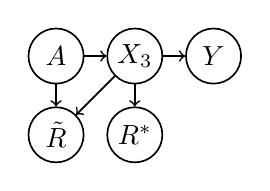
\begin{tikzpicture}[->,auto, semithick, scale=1,every node/.style={scale=1}]
    \tikzset{var/.style={draw=black,circle,minimum size=0.7cm, inner sep=0pt}};
    \node[var] (sX) {$X_3$};
    \node[var, left of=sX] (sA) {$A$};
    \node[var, right of=sX] (sY) {$Y$};
    \node[var, below of=sA] (sR2) {$\tilde R$};
    \node[var, below of=sX] (sR1) {$R^*$};
    {
      \path
        (sA) edge (sX)
        (sX) edge (sY)
        (sX) edge (sR1)
        (sX) edge (sR2)
        (sA) edge (sR2)
        ;
      }
    \end{tikzpicture}
\end{center}
\caption{Graphical model for Scenario II.}
\label{fig:scenario2}
\end{wrapfigure}

Now consider the dependency structure depicted in Figure~\ref{fig:scenario2}. 
Here $X_3$ is a feature, e.g. ``wealth'' or
``annual income'', correlated with the protected attribute $A$ and
directly predictive of the target $Y$.  That is, in this model, the
probability of paying back of a loan is just a function of an
individual's wealth, independent of their race.  Using $X_3$ on its
own as a predictor, e.g.~using the score $R^*=X_3$, does not naturally
seem directly discriminatory.  However, as can be seen from the
dependency structure, this score does {\em not} satisfy equalized
odds. We can correct it to satisfy equalized odds and consider the
optimal non-discriminating predictor $\tilde{R}=\tilde{r}_{II}(X_3,A)$
that does satisfy equalized odds.  If $A$ and $X_3$, and thus $A$ and
$Y$, are positively correlated, then $\tilde{R}$ would depend
inversely on $A$ (see numerical construction below), introducing a
form of ``corrective discrimination'', so as to make $\tilde{R}$ is
independent of $A$ given $Y$ (as is required by equalized odds).

\subsection{Unidentifiability}

The above two scenarios seem rather different.  The optimal score
$R^*$ is in one case based directly on $A$ or its surrogate, and in
another only on a directly predictive feature, but this is not
apparent by considering the equalized odds criterion, suggesting a
possible shortcoming of equalized odds. In fact, as we will now
see, the two scenarios are {\em indistinguishable} using any oblivious
test. That is, no test based only on the target labels, the protected
attribute and the score would give different indications for the
optimal score $R^*$ in the two scenarios. If it were judged unfair in one
scenario, it would also be judged unfair in the other.

We will show this by constructing specific instantiations of the two
scenarios where the joint distributions over $(Y,A,R^*,\tilde{R})$ are
identical. The scenarios are thus unidentifiable based only on these
joint distributions.

We will consider binary targets and protected attributes taking values
in $A,Y\in\{-1,1\}$ and real valued features. We deviate from our convention of
$\{0,1\}$-values only to simplify the resulting expressions.
In Scenario I, let:
\begin{itemize}
\item $\Pr\Set{A=1}=1/2$, and $X_1=A$
\item $Y$ follows a logistic model parametrized based on $A$:
  $\Pr\Set{Y=y\mid A=a} = \frac1{1+\exp(-2ay)},$
\item $X_2$ is Gaussian with mean $Y$: $X_2=Y+{\mathcal N}(0,1)$
\item Optimal unconstrained and equalized odds scores are given by: $R^*=X_1 + X_2=A + X_2,$ and $\tilde{R}=X_2$
\end{itemize}
In Scenario II, let:
\begin{itemize}
\item $\Pr\Set{A=1}=1/2$.
\item $X_3$ conditional on $A=a$ is a mixture of two Gaussians:
  ${\mathcal N}(a+1, 1)$ with weight $\frac1{1+\exp(-2a)}$ and
  ${\mathcal N}(a-1, 1)$ with weight $\frac1{1+\exp(2a)}.$
\item $Y$ follows a logistic model parametrized based on $X_3$: $\Pr\Set{Y=y\mid X_3=x_3}= \frac1{1+\exp(-2yx_3)}.$
\item Optimal unconstrained and equalized odds scores are given by: $R^* = X_3,$  and $\tilde{R}= X_3-A$
\end{itemize}
%
The following proposition establishes the equivalence
between the scenarios and the optimality of the scores (proof at end of section):
\begin{proposition}\label{prop:unident}
  The joint distributions of $(Y,A,R^*,\tilde{R})$ are identical in
  the above two scenarios.  Moreover, $R^*$ and $\tilde{R}$ are
  optimal unconstrained and equalized odds scores respectively, in
  that their ROC curves are optimal and for any loss function an
  optimal (unconstrained or equalized odds) classifier can be derived
  from them by thresholding.
\end{proposition}
\begin{figure}
\centering
  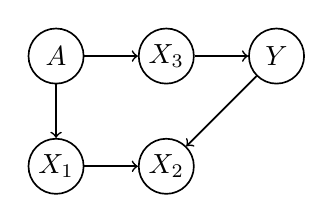
\begin{tikzpicture}[->,auto, semithick, scale=1,every node/.style={scale=1,,node distance = 14mm}]
    \tikzset{var/.style={draw=black,circle,minimum size=0.7cm, inner sep=0pt}};
    \node[var] (sX3) {$X_3$};
    \node[var, left of=sX3] (sA) {$A$};
    \node[var, right of=sX3] (sY) {$Y$};
    \node[var, below of=sA] (sX1) {$X_1$};
    \node[var, below of=sX3] (sX2) {$X_2$};
    {
      \path
        (sA) edge (sX3)
        (sX3) edge (sY)
        (sA) edge (sX1)
        (sY) edge(sX2)
        (sX1) edge(sX2)
        ;
      }
    
    \end{tikzpicture}
  \qquad \qquad  \qquad
  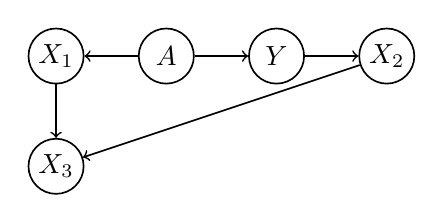
\begin{tikzpicture}[->,auto, semithick, scale=1,every node/.style={scale=1,node distance = 14mm}]
    \tikzset{var/.style={draw=black,circle,minimum size=0.7cm, inner sep=0pt}};
    \node[var] (sA) {$A$};
    \node[var, left of=sA] (sX1) {$X_1$};
    \node[var, right of=sA] (sY) {$Y$};
    \node[var, right of=sY] (sX2) {$X_2$};
    \node[var, below of=sX1] (sX3) {$X_3$};
    {
       \path
        (sA) edge (sX1)
        (sA) edge (sY)
        (sY) edge (sX2)
        (sX2) edge(sX3)
        (sX1) edge(sX3)
        ;
      }
    \end{tikzpicture}

    \caption{Two possible directed dependency structures for the
      variables in scenarios I and II.  The undirected (infrastructure
      graph) versions of both graphs are also possible.}\label{fig:twooptions}
\end{figure}
Not only can an oblivious test (based only on $(Y,A,R)$) not
distinguish between the two scenarios, but even having access to the
features is not of much help.  Suppose we have access to all three
feature, i.e.~to a joint distribution over $(Y,A,X_1,X_2,X_3)$---since
the distributions over $(Y,A,R^*,\tilde{R})$ agree, we can construct
such a joint distribution with $X_2=\tilde{R}$ and $X_3=\tilde{R}$.
The features are correlated with each other, with $X_3=X_1+X_2$.
Without attaching meaning to the features or making causal assumptions
about them, we do not gain any further insight on the two scores.  In
particular, both causal structures depicted in Figure~\ref{fig:twooptions} are
possible.


\subsection{Comparison of different oblivious measures}
%
It is interesting to consider how different oblivious measures apply
to the scores $\tilde{R}$ and $R^*$ in these two scenarios.

As discussed in Section \ref{sec:opt-thresholds}, a score satisfies
equalized odds iff the conditional ROC curves agree for both values of
$A$, which we refer to as having \emph{identical} ROC curves.
\begin{definition}[Identical ROC Curves]
We say that a score $R$ has \emph{identical conditional ROC curves} if
$C_a(t)=C_{a'}(t)$
for all groups of $a,a'$ and all $t\in\mathbb{R}$.
\end{definition}
In particular, this property is achieved by an equalized odds 
score~$\tilde{R}$.
%
Within each protected group, i.e.~for each value $A=a$, the score
$R^*$ differs from $\tilde{R}$ by a fixed monotone transformation,
namely an additive shift $R^*=\tilde{R}+A$.  Consider a derived
threshold predictor $\hat{Y}(\tilde{R})=\ind\set{\tilde{R}>t}$ based
on $\tilde{R}$.  Any such predictor obeys equalized odds.  We can also
derive the same predictor deterministically from $R^*$ and $A$ as
$\hat{Y}(R^*,A)=\ind\set{R^*>t_A}$ where $t_A=t-A$.  That is, in our
particular example, $R^*$ is special in that optimal equalized odds
predictors can be derived from it (and the protected attribute $A$)
deterministically, without the need to introduce randomness as in
Section \ref{sec:opt-thresholds}.  In terms of the $A$-conditional ROC
curves, this happens because the images of the conditional ROC curves
$C_0$ and $C_1$ overlap, making it possible to choose points in the
true/false-positive rate plane that are on both ROC curves.  However,
the same point on the conditional ROC curves correspond to different
thresholds!  Instead of $C_0(t)=C_1(t)$, for $R^*$ we have
$C_0(t)=C_1(t-1)$.  We refer to this property as ``matching''
conditional ROC curves:
\begin{definition}[Matching ROC curves]
We say that a score $R$ has \emph{matching conditional ROC curves} if
the images of all $A$-conditional ROC curves are the same, i.e.,
for all groups $a,a',$
$\set{ C_a(t) \colon t\in\mathbb{R} } = \set{ C_{a'}(t) \colon
  t\in\mathbb{R} }.$
\end{definition}
Having matching conditional ROC curves corresponds to being
deterministically correctable to be non-discriminating: If a predictor
$R$ has matching conditional ROC curves, then for any loss function
the optimal equalized odds derived predictor is a deterministic
function of $R$ and $A$.  But as our examples show, having matching
ROC curves does not at all mean the score is itself
non-discriminatory: it can be biased according to $A$, and a
(deterministic) correction might be necessary in order to ensure
equalized odds.

Having identical or matching ROC curves are properties of the
conditional distribution $R|Y,A$, also referred to as ``model
errors''.  Oblivious measures can also depend on the conditional
distribution $Y|R,A$, also referred to as ``target population errors''.
In particular, one might consider the following property:
\begin{definition}[Matching frequencies]
  We say that a score $R$ has \emph{matching conditional frequencies},
  if for all groups $a,a'$ and all scores $t,$ we have
\[
\Pr\Set{Y=1\mid R=t, A=a} = \Pr\Set{Y=1\mid R=t, A=a'}\,.
\]
\end{definition}
Matching conditional frequencies state that at a given score, both
groups have the same probability of being labeled positive.  The
definition can also be phrased as requiring that the conditional
distribution $Y|R,A$ be independent of $A$.  In other words, having
matching conditional frequencies is equivalent to $A$ and $Y$ being independent
conditioned on $R$.  The corresponding dependency structure is
$Y-R-A$.  That is, the score $R$ includes all possible information the
protected attribute can provide on the target $Y$.  Indeed having
matching conditional frequencies means that the score is in a sense
``optimally dependent'' on the protected attribute $A$.  Formally, for
any loss function the optimal (unconstrained, possibly discriminatory)
derived predictor $\Yhat(R,A)$ would be a function of $R$ alone, since
$R$ already includes all relevant information about $A$.  In
particular, an unconstrained optimal score, like $R^*$ in our
constructions, would satisfy matching conditional frequencies.  Having
matching frequencies can therefore be seen as a property indicating
utilizing the protected attribute for optimal predictive power,
rather then protecting discrimination based on it.

It is also worth noting the similarity between matching frequencies
and a binary predictor $\Yhat$ having equal conditional precision,
that is $\Pr\Set{Y=1\mid \Yhat=\hat{y}, A=a} = \Pr\Set{Y=1\mid
  \Yhat=\hat{y}, A=a'}$.  Viewing $\Yhat$ as a score that takes two
possible values, the notions agree. But $R$ having matching
conditional frequencies does {\em not} imply the threshold predictors
$\Yhat(R)=\ind\set{R>t}$ will have matching precision---the
conditional distributions $R|A$ might be different, and these are
involved in marginalizing over $R>t$ and $R\leq t$.

To summarize, the properties of the scores in our scenarios are:
\begin{itemize}
\item $R^*$ is optimal based on the features and protected attribute,
  without any constraints.
\item $\tilde{R}$ is optimal among all equalized odds scores.
\item $\tilde R$ does satisfy equal odds, $R^*$ does not satisfy equal odds.
\item $\tilde R$ has identical (thus matching) ROC curves, 
  $R^*$ has matching but non-identical ROC curves.
\item $R^*$ has matching conditional frequencies, while $\tilde{R}$
  does not.
\end{itemize}

\subsubsection*{Proof of Proposition \ref{prop:unident}}

  First consider Scenario I.  The score $\tilde{R}=X_2$ obeys equalized
  odds due to the dependency structure.  More broadly, if a score
  $R=f(X_2,X_1)$ obeys equalized odds, for some randomized function
  $f$, it cannot depend on $X_1$: conditioned on $Y$, $X_2$ is
  independent of $A=X_1$, and so any dependency of $f$ on $X_1$ would
  create a statistical dependency on $A=X_1$ (still conditioned on
  $Y$) which is not allowed.  We can verify that
  $\Pr\set{Y=y\mid X_2=x_2} \propto \Pr\set{Y=y}\Pr\set{X_2=x_2\mid Y=y} \propto
  \exp(2y x_2)$ which is monotone in $X_2$, and so for any loss
  function we would just want to threshold $X_2$ and any function
  monotone in $X_2$ would make an optimal equalized odds predictor.

To obtain the optimal unconstrained score consider
\begin{align*}
\Pr\set{Y=y\mid X_1=x_1,X_2=x_2} & \propto
\Pr\set{A=x_1}\Pr\set{Y=y\mid A=x_1}\Pr\set{X_2=x_2\mid Y=y} \\
&\propto\exp(2y(x_1+x_2)).
\end{align*}
That is, optimal classification only depends on
$x_1+x_2$ and so $R^*=X_1+X_2$ is optimal.

Turning to scenario II, since $P(Y|X_3)$ is monotone in $X_3$, any
monotone function of it is optimal (unconstrained), and the dependency
structure implies its optimal even if we allow dependence on $A$.
Furthermore, the conditional distribution
$Y|X_3$ matched that of  $Y|R^*$ from scenario I since again we have
$\Pr\set{Y=y|X_3=x_3}\propto \exp(2 y x_3)$ by construction.  Since we
defined $R^*=X_3$, we have that the conditionals $R^*|Y$ match.  We
can also verify that by construction $X_3|A$ matches $R^*|A$ in
scenario I.  Since in scenario I, $R^*$ is optimal even dependent on
$A$, we have that $A$ is independent of $Y$ conditioned on $R^*$, as
in scenario II when we condition on $X_3=R^*$.  This establishes the
joint distribution over $(A,Y,R^*)$ is the same in both scenarios.
Since $\tilde{R}$ is the same deterministic function of $A$ and $R^*$
in both scenarios, we can further conclude the joint distributions
over $A,Y,R^*$ and $\tilde{R}$ are the same.  Since equalized odds is
an oblivious property, once these distributions match, if $\tilde{R}$
obeys equalized odds in scenario I, it also obeys it in scenario II.
% \end{proof}
